\title{THE DILOGARITHM FUNCTION IN GEOMETRY AND NUMBER THEORY$^{1}$}
\footnotetext[1]{This paper is a revised version of a lecture given in Bonn on the occasion of F. Hirzebruch's 60th birthday, (October 1987) and has also appeared under the title ``The remarkable dilogarithm'' in the Journal of Mathematical and Physical Sciences, 22(1988).}
\markright{The Dilogarithm Function in Geometry and Number Theory}


\author{By~ D. Zagier}
\markboth{D. Zagier}{The Dilogarithm Function in Geometry and Number Theory}

\date{}
\maketitle

\setcounter{pageoriginal}{230}
\textsc{The\pageoriginale dilograrithm Function} is the function defined by the power series
$$
\Li_{2}(z)=\sum\limits_{n=1}^{\infty} \frac{z^{n}}{n^{2}}\quad\text{for~ } |z|<1.
$$

The definition and the name, of course, come from the analogy with the Taylor series of the ordinary logarithm around 1,
$$
-\log (1-z)=\sum\limits^{\infty}_{n=1}\frac{z^{n}}{n}\quad\text{for~ } |z|<1,
$$
which leads similarly to the definition of the {\em polylogarithm}
$$
\Li_{m}(z)=\sum\limits^{\infty}_{n=1}\frac{z^{n}}{n^{m}}\quad\text{for~ } |z|<1, \ m=1,2,\ldots
$$
The relation
$$
\frac{d}{dz}\Li_{m}(z)=\frac{1}{z}\Li_{m-1}(z)\quad (m\geq 2)
$$
is obvious and leads by induction to the extension of the domain of definition of $\Li_{m}$ to the cut plane $\mathbb{C}-(1,\infty)$; in particular, the analytic continuation of the dilogarithm is given by
$$
\Li_{1}(z)=-\int\limits^{z}_{0}\log (1-u)\frac{du}{u}\quad\text{for~ } z\in \mathbb{C}-(1,\infty).
$$
\begin{figure}[H]
\centering
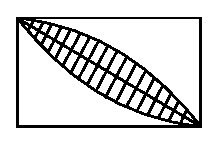
\includegraphics[scale=.9]{figures/fig1.eps}
\end{figure}

Thus\pageoriginale the dilogarithm is one of the simplest non-elementary functions one can imagine. It is also one of the strangest. It occurs not quite often enough, and in not quite an important enough way, to be included in the Valhalla of the great transcendental functions --- the gamma function, Bessel and Legendre 
%page 232
